In applied statistics and machine learning, mixture models are a fundamental tool for treating data taken from multiple subpopulations \cite{ref3}. The data in a mixture model is generated from a number of likely sources, and to identify the nature of the individual sources is one of the goals when dealing with such models. As such, estimating the unknown parameters of the mixture model from sampled data—and particularly, the parameters of the underlying constituent distributions—is an important statistical task. 

The reliability of various partially observable dynamical system models, and latent variable models also depend on successful estimation of the underlying parameters.

For discrete observations, Hidden Markov models have been widely used to represent belief as a discrete distribution over latent states. Under certain controlled conditions, alternate representations (\textit{i.e. Predictive State Representations (PSRs)} \cite{ref30}, \textit{Observable Operator Models(OOMs)} \cite{ref9} ) of Hidden Markov models have also been used for easier inference.

These alternate representations have inspired various spectral learning approaches, which we will look into as we go further down this paper. And coupled with some major advantages such as statistical consistency, easier implementation using simple linear algebra routines, these novel approaches are critically acclaimed day by day. 

Despite these attractive features, many older spectral algorithms are batch methods (needing to store their entire training data set in memory at once) instead of on-line ones.\cite{ref31} However, there are newer algorithms with online learning approaches which can scale to much larger data sets and more complex systems than previous methods.

Although there has been promising progress in parametric cases, where the distribution of the observations conditioned on the latent variables belongs to a parametric family, much is still left to be done for the non-parametric case. 

The rest of the paper is organized as follows: section two gives a general overview of the parameter estimation problem in different latent variable models, in section three we discuss briefly about HMMs and the relevant alternate representations of HMMs, then we move on to section four where we talk about spectral learning approach, including the required framework to develop a spectral learning algorithm, and newer domains that the approach has covered, and in the last section i.e. section five, we discuss the results, concluding with the present limitations, and the possibilities for future work.   


\section{Parameter estimation in latent-variable models}

\subsection{Traditional heuristic methods}

For most mixture models, including the widely popular mixtures of Gaussians and hidden
Markov models (HMMs), current practices rely on the Expectation-Maximization (EM) algorithm,
a local search heuristic for maximum likelihood estimation.

The EM algorithm is a remarkably successful
method for parameter estimation within these models: it is simple, it is often relatively
efficient, and it has well understood formal properties.\cite{ref19} 

It does, however, have a major limitation: it has no guarantee of finding the global optimum of the likelihood function.
From a theoretical perspective, this means that the EM algorithm is not guaranteed to give
statistically consistent parameter estimates. From a practical perspective, problems with
local optima can be difficult to deal with.

Under mild conditions,
the EM algorithm is guaranteed to converge to a local maximum of the log-likelihood
function. This is, however, a relatively weak guarantee; there are in general no guarantees
of consistency for the EM algorithm, and no guarantees of sample complexity, for example
within the PAC framework \cite{ref19}. 

This has led a number of researchers to consider
alternatives to the EM algorithm, which do have PAC-style guarantees.






\subsection{Method of moments}

An alternative to maximum likelihood and EM, especially applicable in the context of mixture models,
is the \textit{method of moments} approach.

The method of moments dates back to the origins of mixture
models, with Pearson’s solution for identifying the parameters of a mixture of two univariate
Gaussians \cite{ref5}. 

The basic paradigm of this approach is simple and intuitive:
\begin{enumerate}[label=\roman*]
\item first, compute certain statistics of the data—often empirical moments such as means and correlations
\item then, find model parameters that give rise to the same (or very close) corresponding population quantities.
\end{enumerate}

To put this in other words, the main idea is to choose model parameters such that it specifies a distribution whose p-\textit{th} order moments - for several values of p- are equal to the corresponding empirical moments observed in the data.

In many different cases, the \textit{method of moments} leads to consistent estimators which can be efficiently computed. This can be relevant particularly when talking of latent variable models, where standard maximum likelihood approaches are typically computationally prohibitive, and heuristic methods can be unreliable and difficult to validate with high-dimensional data. 


Since Pearson’s work, the \textit{method of moments} has been studied
and adapted for a variety of problems, and the method has been favored to a certain extent because it guarantees statistical consistency under mild conditions.

But the method often runs into trouble with large mixtures of high-dimensional distributions. This is because the equations determining the parameters are typically based on moments of order equal to the number of model parameters, and high-order moments are very difficult to estimate accurately due to their large variance.

To address this issue, Anandkumar et al. \cite{ref6} developed a computationally efficient \textit{method of moments} based on only low-order moments that can be used to estimate the parameters of a broad class of high-dimensional mixture
models with many components. As such, the resulting estimators can be implemented with standard numerical
linear algebra routines (singular value and eigenvalue decompositions), and the estimates have
low variance because they only involve low-order moments.
The class of models covered by the method includes certain multivariate Gaussian mixture models and HMMs, as well as mixture models with no explicit likelihood equations.

In the following sections, we will go on to see how this idea of method of moments has been used to develop efficient spectral algorithms to estimate parameters in latent variable models (in this work however, we will especially focus on Hidden Markov Models).



\section{Background and related work}

\subsection{Brief overview on Hidden Markov Models}

\subsubsection{HMMs for modeling discrete time- series data}

When it comes to statistical model for discrete time series data, Hidden Markov Models (HMMs) \cite{ref1} are one of the most popular models with applications as diverse as automatic speech recognition, natural language processing (NLP), and genomic sequence modeling. 

In a Hidden Markov model, a discrete hidden state evolves according to some Markovian dynamics, and observations at a particular time depend only on the hidden state at that time\cite{ref2}.\newline
HMM is a good example of a latent variable model which assumes
that sequential data points are noisy, incomplete observations
of a latent state that evolve over time.
The distributional assumptions of HMMs result
in important differences in the evolution of their belief
over time.

The discrete state of HMMs is good for modeling systems with \textit{competitive inhibition} \cite{ref7}: e.g., a
HMM can predict that our next observation will be either image A or image B, while disallowing blends of A and B. \newline
\newline
However, when it comes to smooth state evolution, HMMs can only model it by discretizing the state space very finely. 
Ideally, it would be desirable to model both \textit{competitive inhibition} and \textit{smooth evolution}, but very few models display both of these properties.

\subsubsection{Alternate representations for HMMs}

There are some models which are capable of both(\textit{competitive inhibition} as well as \textit{smooth evolution}), i.e. \textit{Switching State Space
Models}\cite{ref8}, which typically rely
on on \textit{approximations} for inference and learning, and are plagued by problems of local optima, especially in large state spaces.
\par

To address these issues, there have been attempts to introduce new novel generalisations of HMMs such as: \textit{Observable Operator Models
(OOMs)} \cite{ref9}, and \textit{Predictive State Representations
(PSRs)} \cite{ref10}. These models represent states as vectors of predicted probabilities of future events (characteristic events) conditioned on past events (indicative
events). 

As these representations are observable, it is believed that efficient, consistent spectral
learning algorithms for PSRs and OOMs are possible. 

But, despite much research in this area there is still a lack of provably accurate learning algorithms that have been demonstrated to work well in practice.

And hence, until recently, the dominant learning algorithms for HMM are all based on local search heuristics i.e. the Baum-Welch / EM algorithm.


\section{Spectral learning approach: a new direction}

This line of work started when Hsu et al.\cite{ref2}
developed a spectral algorithm for HMMs which could learn observable representations of HMMs. This method recovers a HMM’s parameters, up to a linear transformation, using singular value decomposition and other simple matrix operations.
\newline
\newline
The work borrows idea from two seemingly unrelated fields and tries to apply them to the learning problem.
\newline
\newline
The first idea,\textit{subspace identification}, is borrowed from the subspace identification literature in control theory \cite{ref12} \cite{ref13}. 
\newline
\subsection{Subspace Identification}

The subspace identification methods, generally used in control theory, use spectral approaches to discover the relationship between hidden states and the observations. In this context, the relationship is
discovered for linear dynamical systems such as Kalman filters. The principal idea being that the relationship between observations and hidden states can often be discovered by spectral/SVD methods correlating the past and future observations (in particular, such methods often do a \textit{Canonical
Correlation Analysis (CCA)}\cite{ref14} between the past and future observations).

However, algorithms presented in the above literatures cannot be directly
applied to learn HMMs because they assume additive noise models with noise distributions independent of the underlying states, and such models are not suitable for HMMs.

In their work, Hsu et al.\cite{ref2} use the idea of performing a CCA between past and future observations to uncover information about the observation process (this is done through
an SVD on a correlation matrix between past and future observations).

To avoid the state-independent additive noise condition, Hsu et al.\cite{ref2} take the help of a second idea, \textit{Observable Operator Models (OOM)}, which we will discuss below.

\subsection{Observable representations of HMM}

Typical strategies for learning HMMs begin by estimating the observation probabilities and the transition probabilities for each hidden state (for instance, by maximizing the likelihood of a certain sample).

But, as the hidden states are not directly observed by the learner, one often resorts to heuristics (e.g. EM) that alternate
between adjusting the hidden states and selecting appropriate parameters that maximize the likelihood of the sample and current state estimates. 

Such heuristics require careful initialization (i.e. an accurate guess of the hidden states) to get the desired outcome, and therefore a better alternative would make things much simpler. 

This brings us back to the idea of observable representation of Hidden Markov models, which we briefly mentioned in a section above.

Rather than explicitly modeling the hidden states, the probabilities of sequences of observations can be represented as products of matrix observation operators. This idea is not a new one and dates back to
the literature on multiplicity automata \cite{ref15} \cite{ref16}.

For simplicity, we define a condition, say Condition A, such that the state Transition Probability Matrix, and Observation Probability Matrix are less than \textit{m}, where \textit{m} is the number of hidden states. This is simply a precautionary measure to exclude some cases under the general learning problem which has been shown to be hard under \textit{cryptographic assumptions} \cite{ref18}, and are far off from those that we are likely to encounter in practical applications.



Under Condition A, HMMs admit an efficiently learnable parameterization that depends
only on observable quantities. Because such quantities can be estimated from data, learning
this representation avoids any guesswork about the hidden states and thus allows for algorithms
with strong guarantees of success.


This idea was also reused, in the Observable Operator Model and the Predictive State Representations that we mentioned above.

The work on Observable Operator Model provides a non-iterative algorithm for learning HMMs, with an asymptotic analysis. 
However, this algorithm assumes prior knowledge of a set of ‘characteristic events’, which implies some relationship between the hidden states and observations.

In \cite{ref2} however, this problem of prior assumption is avoided by making use of first idea mentioned above.


Within the community, there has been one another effort,\cite{ref17},  which has successfully managed to learn HMMs (with PAC-style guarantees of sample complexity), which also relies on the same rank condition and computation similar to \cite{ref2}. However, the work fails to address large observation spaces, and thus the algorithm assumes the state and observation spaces to have the same dimension. In addition, it takes the approach of learning the observation and transition matrices explicitly, which results in a less sample-efficient algorithm.

This problem is addressed in \cite{ref2}, where the \textit{explicit} recovery of the observation and transition matrix is avoided, and instead \textit{subspace identification} is used to learn alternative representation.

\subsection{Spectral algorithm for estimating HMMs}

By applying spectral methods, Hsu et al.\cite{ref2} were able to develop an algorithm free of local optima and statistically consistent, which has a finite-sample bound on L1 error in joint probability estimates. 

However, learning large-statespace HMMs is still difficult: the number of parameters
grows prohibitively with the size of the state space.

To address this problem, \cite{ref7} extends the advantages of spectral
learning to a larger class of models using a variant of HMMs called Reduced-Rank HMMs (RRHMMs), which have a large implicit state space but a low-rank transition matrix.

Using the same idea of observable representation as discussed above, the parameters are estimated using Singular Value Decomposition (SVD).


Here, the basic algorithm for estimating rank-k RR-HMMs is
equivalent to the spectral learning algorithm of \cite{ref2} for learning k-state HMMs. But the improvement here is the relaxation of the conditions, for instance in \cite{ref2} a full-rank transition matrix was the basic assumption, without which the bounds were vacuous. This leniency of the conditions lead to finite-sample performance guarantees for rank-k RR-HMMs.
\newline
\newline
The algorithm derived on \cite{ref7}, improved upon the work \cite{ref2}, can be described as follows:

The algorithm takes as input the desired rank \textit{k}
rather than the number of states \textit{m}, as was done in \cite{ref2}.

Alternatively (as seen on step 2 of the algorithm below), given a threshold, the algorithm can choose the rank of the HMM by examining the singular values of \[\widehat{{P}_{2,1}}\]
 \quad where, $ \widehat{{P}_{2,1}} $ is the covariance matrix whose rank is \textit{k} in the absence of noise. 

It assumes that we are given \textit{N} independently sampled
observation triples $\langle x1, x2, x3\rangle$ from the HMM. 
The algorithm results in an estimated observable representation of the RR-HMM:
\newline
\begin{figure}[h]
    \centering
    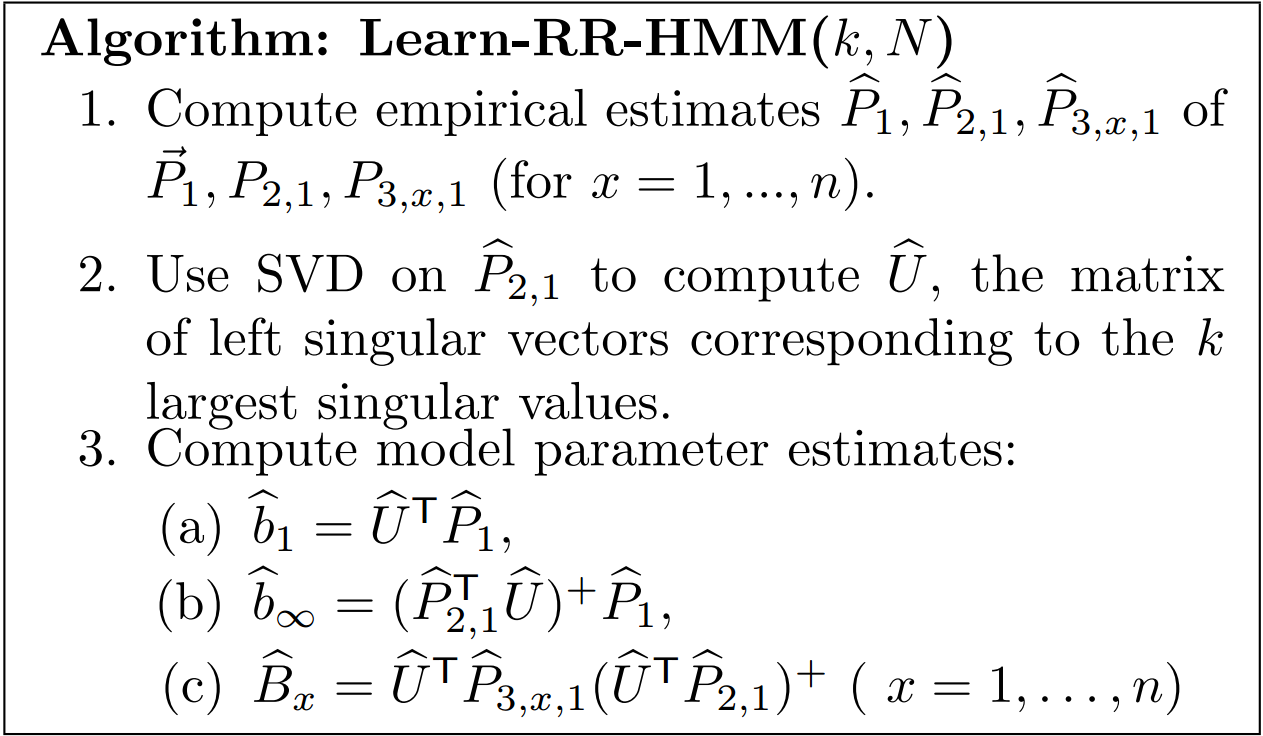
\includegraphics[scale=0.2]{algorithm_RRHMM.png}        
\end{figure}

where, ${\vec{P}_{\,1}}$, is the initial probability vector,
$ {P}_{2,1} $ is the covariance matrix, and
$ {P}_{3,x,1} $ is the trivariance matrix

\textbf{Note}: The detailed workout of the algorithm can be found in \cite{ref7}.


The probability matrix $ {P}_{2,1} $  acts as a correlation matrix relating one past timestep to one future timestep.

As such, it is possible to consider \textit{sequences of
observations} in the past and future and estimate larger
versions of $ {P}_{2,1} $  and $ {P}_{3,x,1} $  accordingly (for single observations
x). These matrices will have one row for each
distinct sequence of past observations, and one column
for each distinct sequence of future observations, and works well as long as the past and future sequences do not overlap.


Another interpretation of $ {P}_{2,1} $,$ {P}_{3,x,1} $, which have been successfully applied in other similar works, is as matrices containing expected values of products of indicator functions of observations, which correspond to simple \textit{indicative} and \textit{characteristic} events \cite{ref9},
or \textit{histories and tests} \cite{ref10}.


\subsection{Extending spectral algorithm to kernel based methods}

As we saw in the preceding sections, the work of Hsu et al.\cite{ref2} has shown that spectral learning algorithms can be used as a viable alternative to local search heuristics for most practical cases. Building upon this, Siddiqi et al.\cite{ref7} generalized the spectral learning algorithm
and bounds of \cite{ref2} to accurately learn
a larger class of sequential data models (RR-HMMs)
under a larger class of observation models (especially non-1-stepobservable domains).


However, these spectral algorithm are only formulated
for HMMs with discrete observations.
In reality, many sources of sequential data are continuous or structured, and hence the spectral algorithm does not apply to such data without discretization and flattening.

As the ultimate goal is to have a universal spectral method that can include all the cases, Song et al.\cite{ref20} came up with a new kernel based
representation and kernelized spectral learning
algorithm for HMMs. This new representation and algorithm widely increases the scope of spectral methods as it allows to learn HMMs in any domain where a kernel can be defined. 


The work depends on the idea of representing HMMs using a 
concept called Hilbert space embedding \cite{ref21} \cite{ref22}. 

The essence of Hilbert space embedding is to represent probability measures (in this case, corresponding to distributions over observations and latent states in a HMM) as points in Hilbert spaces. 

After that, inference can be done in the HMM by updating these points, entirely in their Hilbert spaces, using covariance operators \cite{ref23} and conditional
embedding operators \cite{ref24}. By making use of the Hilbert space’s metric structure, this method works naturally with continuous and structured
random variables, without the need for discretization.

This is an improvement over previous work by Song et al.\cite{ref24} where a kernel algorithm was derived for HMMs. However, they only provided results for fully observable models, where the training data includes labels
for the true latent states. By contrast, the algorithm presented in \cite{ref20} only requires access to an (unlabeled) sequence of observations.

In the next section, we will see how this new learning algorithm (referred from now on as embedded HMM) fares compared to other methods in real world filtering and prediction tassks.